%\documentclass[12pt,a4j]{jreport}
\documentclass[a4paper,11pt]{jreport}
%\usepackage[dvips]{graphicx,color}
%\usepackage{array}main
%\usepackage{amsmath,amsthm,amssymb}
%\usepackage{refcheck}
%%%%%%%%%%%%%%%%%%%%%%%%%%%%%%%%%%%%%%%%%%%%%%%%%%%%%%%%%%%%%%%%%%%%
%\usepackage{eepic,eepicsup}
\setlength{\columnsep}{4mm}
\setlength{\parskip}{1.4mm}


%\documentclass[twocolumn]{jarticle}
%\usepackage{sea-ss}head
%\documentcl$AS$s{jarticle}
%\usepackage{twocolumn}
%\usepackage{multicol}
%\usepackage{sea-ss}
\usepackage[dvipdfmx]{graphicx}
\usepackage{url}
%\usepackage{epsfig}
\usepackage[fleqn]{amsmath}
%\usepackage[varg]{txfonts}
%\usepackage{float}
\usepackage{caption}
\usepackage{flushend}

%excel2latex用に追加
\usepackage{multirow}
\usepackage{bigstrut}


%筑波大学のフォーマットからコピー
\usepackage{times} % use Times Font instead of Computer Modern

\setcounter{tocdepth}{3}
\setcounter{page}{-1}

\setlength{\oddsidemargin}{0.1in}
\setlength{\evensidemargin}{0.1in}
\setlength{\topmargin}{0in}
\setlength{\textwidth}{6in}
%\setlength{\textheight}{10.1in}
\setlength{\parskip}{0em}
\setlength{\topsep}{0em}
%%%%%%%%%%%%%%%%%%%%%%%%%%%%%%%%%%%%
%% タイトル生成用パッケージ(重要)
%\usepackage{sie-jp-sjis}
\usepackage{sie-jp-utf}

%% タイトル
%% 【注意】タイトルの最後に\\ を入れるとエラーになります
\title{入出力データの順序情報に基づくブラックボックステスト手法に関する研究}
%\title{A study on the method of blackbox testing based on I/O data sequence}
%% 著者
\author{湯本剛}
%% 学位 (2012/11 追加)
%\degree{}
%% 指導教員
%\advisor{}

%% 専攻名 と 年月
%% 年月は必要に応じて書き替えてください。
%\majorfield{△△△△}\programfield{□□□□}
\yearandmonth{2018年 3月}
%%%%%%%%%%%%%%%%%%%%%%%%%%%%%%%%%%%%%%%%%%%%%%%%%%%%%%%%%%%%%%%%%%%%

\begin{document}

\maketitle
\thispagestyle{empty}
\newpage

\thispagestyle{empty}
\vspace*{20pt plus 1fil}
\parindent=1zw
\noindent
%%
%% 論文の概要(Abstract)
%%
\begin{center}
{\bf 概要}
\vspace{5mm}
\end{center}
本研究はブラックボックステストのテストケース抽出に抜け漏れやケース数が増 大する課題に対して,
テスト対象に対する入出力データの順序情報に基づいてテストケースを抽出する 手法を提案し,合理的に
テストケースを抽出することを成果とするものである.
%%%%%
\par
\vspace{0pt plus 1fil}
\newpage

\pagenumbering{roman} % I, II, III, IV
\tableofcontents
\listoffigures
%\listoftables

\pagebreak \setcounter{page}{1}
\pagenumbering{arabic} % 1,2,3

%%%%%%%%%%%%%%%%%%%%%%%
\chapter{序論}
ソフトウェア開発において,開発したソフトウェアの品質を確保する主要な工程にソフトウェアテストがある.
日本におけるテスト工数の割合は開発工数全体の28パーセントから35パーセントを占める場合が多いが,90パーセントを超える場合もあるという調査結果が出ている\cite{IPA2015}.
ソフトウェアテストの活動のうち,テスト実行工程がソフトウェア開発のクリティカルパス上にある唯一の工程となる.
テスト実行の前にテストケースを開発し,実行するテストの全体像を示せると,効率のよいテスト実行を計画できる.
効率のよいテストとは,テストの効果に対するリソースが少ないことである.
また,テストを行うことで十分に品質を行うためには,重複が無く抜け漏れの無いテストケースを開発することが重要になる.
求められるテストケースの数は,昨今のソフトウェアの複雑性と規模の急激な増加に伴い増加の一途をたどっている.
ブラックボックステストの場合,ソフトウェアの規模とテストケース数の関係は,ファンクションポイント総計値の1.15乗から1.3乗となる\cite{jones1998estimating}.また,開発プロジェクトのファンクションポイント総計値は1970年から2000年までの30年間で約10倍の増加を示している\cite{longstreet2000}.
また,組み込みソフトウェア開発のソフトウェア規模の増加は,ドメインによって毎年10パーセントから20パーセントに及ぶという調査結果もある \cite{jones2009}.
テストケース数の増加に対応するために必要となるテスト工数は,ソフトウェア開発工数の多くを占めるようになってきている.

また,テストケースを作成する工数は,平均的にテスト工数全体の40パーセントだと言われている\cite{van2013tpi}.
これは,テストケースの開発に多くの人員が必要となることを示している.
日本では,複数のシステムを統合するといった大規模な開発にて8ヶ月の間に約5000人がテストに投入されたという事例もある\cite{2009システム統合の}.
多数の人員がテストケースを作成する工程に必要とされているにもかかわらず, テストケースを作成するための明確に定義されたルールがないために,投入された人員は個々の考え方に基づいてテストを開発することが多い.
これはテストケースの重複や漏れの原因となり,テストの活動がソフトウェアの品質を確保する役割を果たせないばかりか,コスト増や納期遅延の原因となる.
本研究では,テストケースを作成する工程に投入される人員が、必要なテストケースを網羅的に抽出し,抜け漏れを防止できるようにすることを目的とし,適切な数のテストケースを開発するための手法を提案し,その適用評価を行う.

本論文は6章で構成される.
2章では,システムテストにおけるブラックボックステストにおける課題と,関連する先行研究について述べる.また,本研究で使用するテスト分析手法について解説する.
3章では,前章で述べた課題を更に分析するために,実験を行い実験結果で確認を行った.
4章では,テストデータの入出力に着目し、テスト対象の分析を網羅的に行う手法の提案と適用評価を行った.
5章では,テストデータの入出力を順番に組み合わせる必要がある際に,重要な順序組み合わせを抽出してテストケースにする方法の提案と適用評価を行なった.
最後の6章では,結論を述べる.

%%%%%%%%%%%%%%%%%%%%%%%
%%%%%%%%%%%%%%%%%%%%%%%
\chapter{システムテストにおけるブラックボックステストの課題}
\section{本研究の対象となるテストケースの開発方法とテストのレベル}
%−−−-図1を入れる
\begin{figure}[htbp]
  \begin{center}
  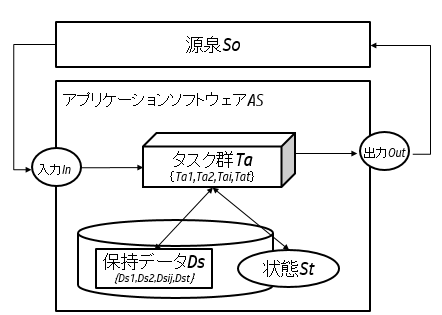
\includegraphics[width=10cm]{./image/fig-1.png}
  \caption{アプリケーションソフトウェアの構成}
  \label{fig:fig-1}
  \end{center}
\end{figure}

\subsection{対象とするアプリケーションソフトウェアの構成}
一般的なアプリケーションソフトウェアは,入力$In$に対して,何らかの出力$Out$を返す.
ソフトウェアの機能は,何らかの入力を出力に変換する処理により実現されていると考えられる.
この処理を本論文ではタスクと呼ぶ.
タスクは,該当のテストレベルからみた入力を出力に変換している1処理である.
そのため,タスクの粒度は,後述するテストレベルによって決まる.%1-3対応
ソフトウェアの構成要素であるタスク$Ta$の出力について考えると,$Ta$への入力$In$だけでなく状態$St$と保持データ(データベースや内部メモリに保存されているデータ)$Ds$の影響を受けると考えられる.
例えば,Webアプリケーションにて予約を行うタスクについて考えると,予約が可能か否かを示す状態と,予約オブジェクトの予約状況を示す保持データによって,予約の成否が決まる.
本論文では,対象として図\ref{fig:fig-1}に示すような状態と保持データを持つアプリケーションソフトウェア($AS$)のタスクに対するテストを研究対象にする.
$AS$の構成要素は,タスク群$Ta$と状態$St$と保持データ$Ds$とし,各タスクは外部の源泉$So$からの入力$In$と$So$への出力$Out$があるとする.
タスク群$Ta$は,その要素を$Ta=\{Ta_1,Ta_2,\cdots,Ta_i,\cdots,Ta_t \}$とし, 対応する入出力は$In_i$と$Out_i$とする.

\subsection{テストケースを開発する方法}
テストケースを開発する方法は,ソフトウェアの物理的な構造を基にテスト設計をするホワイトボックステストと,ソフトウェアの仕様を基にテスト設計をするブラックボックステストに大別できる\cite{myers2011art} .
ホワイトボックステストはテスト設計のベースがソースコードのようなテスト対象そのものとなるため,テスト対象プログラムの行を網羅,分岐を網羅といった具合にテストにて網羅すべきアイテムを明確に選択することが容易である.
網羅基準はテスト設計技法として提唱されている[2].
一方,ブラックボックステストでは,テスト対象そのものではなく,テスト対象の動作条件や振る舞いについて記述した仕様をベースにしてテストケースを開発する.
ブラックボックステストのテスト設計技法の中で、仕様に対する網羅基準は,ホワイトボックステスト同様,数多く提唱されている[2].
しかし,ブラックボックステストは,テストベースがテスト対象の物理的な構造ではなく論理的なふるまいの記述であるがゆえに,テストを作るための詳細化が複数の解釈で行われることが多い.
結果的にテストケースの重複や抜け漏れを引き起こす可能性も高くなる.
本研究では,ブラックボックステストを対象とする.

\subsection{テストレベル}

\begin{figure}[htbp]
  \begin{center}
  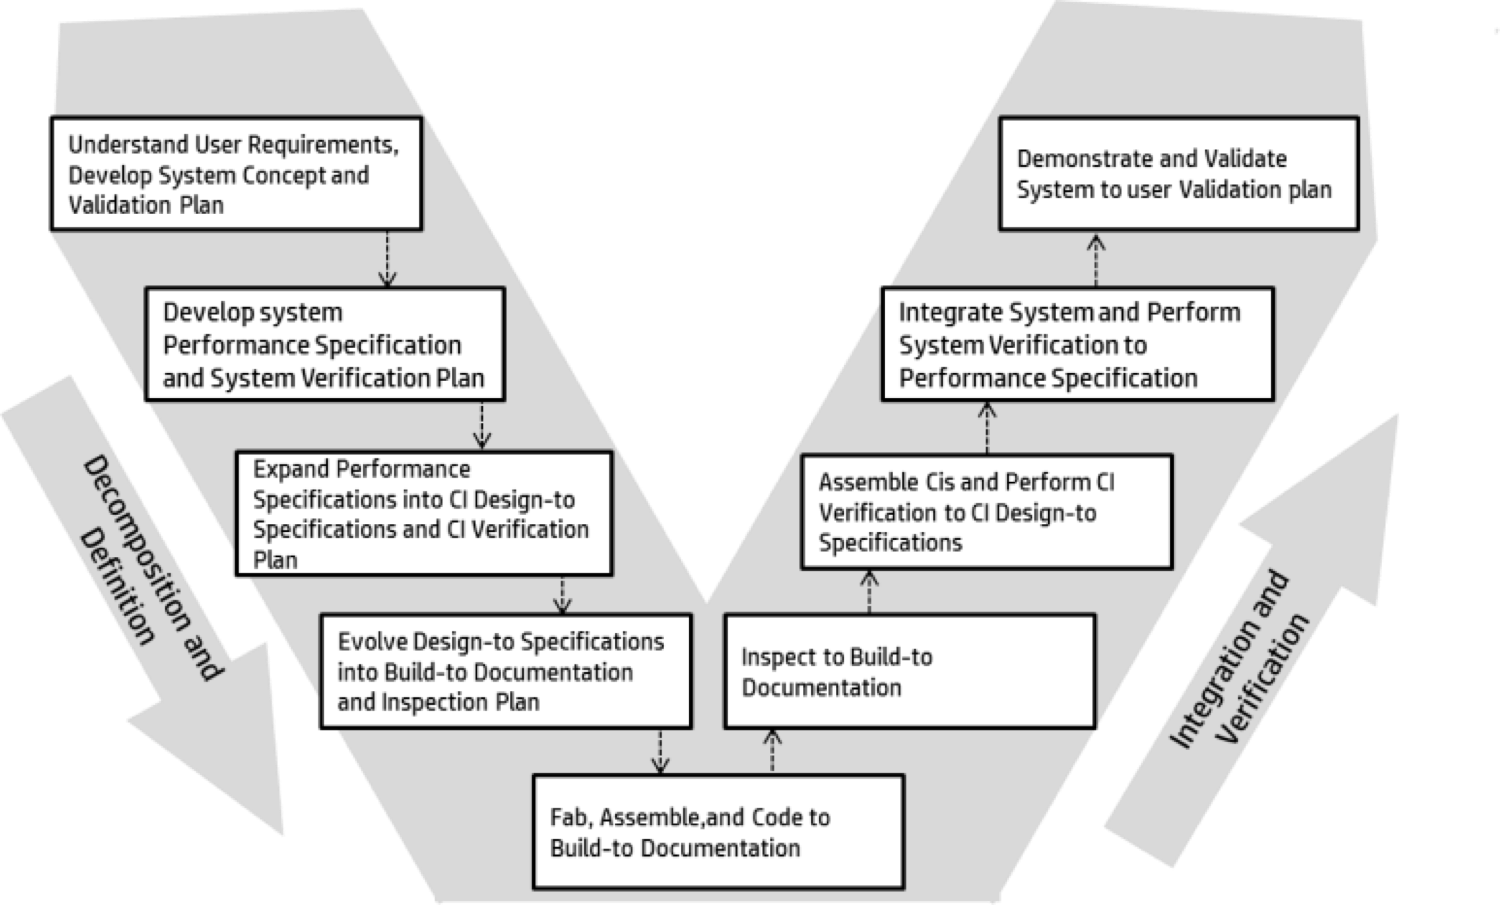
\includegraphics[width=10cm]{./image/D-2-Fig1.png}
  \caption{Vモデル}
  \label{fig:D-2-Fig1}
  \end{center}
\end{figure}
ソフトウェアテストは,開発ライフサイクルの中で複数のテストレベルに分けて行われる.
複数のテストレベルは,図~\ref{fig:D-2-Fig1}で示すVモデルと呼ばれる技術面にフォーカスしたライフサイクルモデルにて表現することができる\cite{forsberg1991}.
各テストレベルはソフトウェア開発の段階的詳細化のレベルと対応している.
テストのプロセスは,Vモデルであらわす各レベルごとに行われる.
本研究は,複数のレベルの中で,図~\ref{fig:D-2-Fig1}の上から2番目の箱となる,「Develop System performance specification and System verification plan」と「Integration system and Perform system verification to performance specificetion」のレベル,つまりシステムレベルのテストで行われるブラックボックステストに焦点を当てている.
システムレベルのテストは,開発した単体のソフトウェアがすべて統合されるため,規模の増大と複雑性の増加の影響を直接的に受けるからである.

\subsection{テスト開発プロセス}
Vモデルであらわす各レベルにて行われるテストはそれぞれ,開発プロセスと類似したプロセスを持っている\cite{ISTQB}.
テストのプロセスは, 図~\ref{fig:D-2-Fig1}「 」のようにテスト計画がVモデルの左側の活動と並行に行われ,その後時系列にテスト分析,テスト設計,テスト実装が行われた後,Vモデルの右側の活動の中で,テスト実行と終了基準の評価が行われる.
テストのプロセスの中でテスト分析,テスト設計,テスト実装の3つのテストケースを作成するための活動はテスト開発プロセスと呼ばれている\cite{ISTQB}.
本研究では,テスト開発プロセスの中のテスト分析とテスト設計を対象とする.
テスト分析では,テスト対象をテスト設計ができるサイズに詳細化する.
ブラックボックステストでのテストを開発するベースは対象とするアプリケーションソフトウェアの仕様である.
仕様とは,図~\ref{fig:D-2-Fig1}で示したVモデルの左側の成果物のことである.
各レベルでテスト設計のベースする仕様はテストベースと呼ばれている.
本研究の対象となるテストレベルでは,「Develop System performance specification and System verification plan」のテストベースに対して,何らかの考え方に基づき,テストにて網羅すべきアイテムを選択し,整理する.
テスト分析でのアウトプットはテスト条件と呼ばれている.
このテスト条件を合理的にある基準で網羅する方法を考える行為がテスト設計であり,そのための技法をテスト設計技法と呼ぶ.
テスト設計のアウトプットはテストケースである.
テストケースは,IEEE610において,特定の目的のために開発されたテスト入力,実行条件,期待結果の3つで構成されると定義している.
また,機能テストは,選択した入力と実行条件のレスポンスとして生成されたアウトプットを確認する,と定義している[2].
すなわち,タスクに対するテストとは,テスト入力,実行条件,を入力して生成されたアウトプットが期待結果と一致するかを確認することである.
このプロセスを図示すると,図1のようになる.
テスト入力,実行条件には,事前に設定されているものと,実行時点で設定するものがある.
本研究では,おのおのを表1に示すよう定義する.
その上で,事前入力と事前条件をまとめたものをテストパラメータ,イベントと操作をまとめたものをテストアクションと呼ぶこととする.

\section{システムレベルでのブラックボックステストの課題} \label{sec:2-2}
\subsection{テストケースの抜け漏れが起きる課題と関連する先行研究}
テスト分析の活動の出力となるテスト条件は,機能,トランザクション,品質特性,構造的要素といったアプリケーションソフトウェアの側面の総称である.
テスト分析では,テスト対象をテスト設計ができるサイズに詳細化する際にこれらの側面に着目して詳細化を行う.
その際は,テスト対象の詳細化をするときの起点や中間分類が人によって異なってバラバラになってしまわなように各側面の関係を整理する必要がある.
しかし,テスト分析におけるテスト条件群の整理方法は,研究や実務においても,経験則や個人の考え方に基づいている.
一般的には,テストベースを大項目,中項目,小項目と詳細化していくことが多い.
この方法は,詳細化する際の各分類項目に当てはめるアプリケーションソフトウェアの側面に明確なルールが定義されていないため,個人毎の何かしらの考え方で詳細化するための分類を決めていくことになる.
そのため,複数人で作業を行うと分類にばらつきが発生し,同じテスト条件が複数の階層に現れてしまったり,同じ意味のテスト条件が別の名称で選択されるといった混乱が起きてしまう.
混乱が起きている例を表~\ref{tab:analysissample}に示す.
% Table generated by Excel2LaTeX from sheet '論文挿絵'
\begin{table}[htbp]
  \centering
  \caption{Add caption}
    \begin{tabular}{|l|l|l|l|l|p{9.335em}|}
    \hline
    大項目   & 中項目   & 小項目   & 細目    & 補足項目  & テスト条件 \bigstrut\\
    \hline
    印刷    & 設定    & 印刷部数  & ー     & ー     & 100部印刷した場合 \bigstrut\\
    \hline
    設定    & プリント設定 & 一般    & 異常系   & エラーメッセージ & 「印刷部数が99部を超えました」と表示されること \bigstrut\\
    \hline
    \end{tabular}%
  \label{tab:analysissample}%
\end{table}%
表~\ref{tab:analysissample}の例には以下のような問題がある.
\begin{enumerate}
\item 設定というカテゴリが大項目に出ている場合と中項目に出ている場合が混在している.
\item 階層数も一定でないため,各階層がどのような意味を持つものかがばらついている.
\item 上段は,期待結果が書かれていない.
\item 上段と下段は同じテスト条件について書かれている.
\end{enumerate}
テスト開発の最初の活動であるテスト分析にて特定するテスト条件にこのような問題があると,その後の活動で作られるテストケースの抜け漏れ,重複に影響を及ぼす.
ISTQBでは,テスト分析は「…テスト分析の期間中,何をテストするか決定するため,すなわち,テスト条件を決めるために,テストのベースとなるドキュメントを分析する [7] 」と説明されている.
ISTQBでは,この説明のとおり,テスト分析を実行するための要求事項や必要性は述べているけれども,テストベースを分析していくためのアプローチは定義されていない.
これは,Ostrand [ ], Grindal [ ]などのテスト開発に関する先行研究でも同様である.
更に言うと,G.J.MyersやB.Beizerといった先行研究の多くは,テスト分析にてテスト条件が特定された後のテスト設計で行われるテストパラメータの設計に焦点を当てている.
そのため,テスト条件は,すでに全て準備されたと言う前提になっている.
それらの研究はテスト分析手法の論理に着目をしているけれども,複数の人数でテスト分析を行う際のテスト条件の重複と欠落について,手法を適用すると実際はどの程度効果的であるかについては,大きく着目していない.
テスト分析手法に関する研究は,Nishi\cite{nishi2012based}, Akiyama\cite{Akiyama2014}, Yumoto\cite{yumoto2013test}がある.
しかし,複数の人数でテスト分析を行う際のテスト条件の重複と欠落について手法がどの程度有効であるかは,ほとんど研究されていない.

\subsection{テストケース数が増えてしまう課題と関連する先行研究}
テストケース数の増加は,単一機能のテストより機能間の統合において問題となる.
この場合のテストケース数は,単一の機能や制御構造の和で求めるのではなく,積となるためである.
それに加え,このテストでは,状態遷移に伴う時系列の組合せのテストも求められることから,テストケース数の爆発問題が生じる.しかし,必要なテストケースの抽出方法とその網羅性に関する研究は多々あるが,多くは機能や制御構造を基にした方法である.\cite{myers2011art}

状態遷移間の組合せについては,N スイッチカバレージに従ってテストケースを抽出する方法がある. \cite{beiz90}
N スイッチカバレージとは,状態の遷移をパスとし,N+1 個の遷移パスを網羅する基準に従て組合せテストケースを作成する.
N=0 では遷移パスの組合せをテストできないため N=1,すなわち S1 網羅基準(1 スイッチカバレージ)が必要とされている.
